\documentclass[11pt,a4paper]{article}
\usepackage[margin=2.2cm]{geometry}
\usepackage{fontspec}
\setmainfont{TeX Gyre Pagella}
\setmonofont{DejaVu Sans Mono}[Scale=0.82]
\usepackage{amsmath,amssymb,amsthm}
\usepackage{graphicx,xcolor,listings,booktabs,enumitem}
\usepackage[most]{tcolorbox}
\usepackage{tikz}
\usepackage{needspace}
\usepackage[hidelinks]{hyperref}

\definecolor{accent}{HTML}{2B6CB0}
\definecolor{warn}{HTML}{C53030}
\newtcolorbox{keybox}[1][]{colback=accent!5,colframe=accent,boxrule=0.6pt,arc=2pt,left=6pt,right=6pt,top=4pt,bottom=4pt,#1}
\newtcolorbox{warnbox}{colback=warn!5,colframe=warn,boxrule=0.6pt,arc=2pt,left=6pt,right=6pt}

\lstdefinelanguage{Rust}{
  keywords={fn,let,mut,if,else,for,in,while,return,use,pub,struct,impl,loop,break,Some,None,as,match,const,Self,self},
  morekeywords=[2]{usize,i32,i64,u64,f64,bool,Vec,VecDeque,BTreeSet,BTreeMap,BinaryHeap,Option,str},
  sensitive=true, morecomment=[l]{//}, morestring=[b]"}
\lstset{language=Rust,basicstyle=\ttfamily,keywordstyle=\color{accent}\bfseries,
  keywordstyle=[2]\color{teal},commentstyle=\color{gray}\itshape,stringstyle=\color{warn},
  frame=single,rulecolor=\color{gray!40},backgroundcolor=\color{gray!4},
  numbers=left,numberstyle=\tiny\color{gray},xleftmargin=1.5em,breaklines=true,
  columns=fullflexible,keepspaces=true,showstringspaces=false}

\newtheorem*{invariant}{Invariant}
\theoremstyle{definition}\newtheorem*{definition}{Definition}

\usepackage{soul}
\definecolor{hlY}{HTML}{FFF3A0}\definecolor{hlG}{HTML}{C8F2C2}\definecolor{hlP}{HTML}{E6D2F7}\definecolor{hlB}{HTML}{CFE3FF}
\newcommand{\hly}[1]{{\sethlcolor{hlY}\hl{#1}}}
\newcommand{\hlg}[1]{{\sethlcolor{hlG}\hl{#1}}}
\newcommand{\hlp}[1]{{\sethlcolor{hlP}\hl{#1}}}
\newcommand{\hlb}[1]{{\sethlcolor{hlB}\hl{#1}}}
\newcommand{\img}[3]{\begin{center}\begin{minipage}{\linewidth}\centering\fcolorbox{gray!50}{white}{\includegraphics[width=#1]{board/#2}}\\[-2pt]{\footnotesize\textcolor{gray}{#3}}\end{minipage}\end{center}}
\newcommand{\extra}{\textsuperscript{\textcolor{warn}{[extra]}}}
% pages of the prof's 2025 notes on the segment tree (Lessons/L13/Segment_tree_2025.pdf)
\newcommand{\stnote}[2]{\begin{center}\fcolorbox{gray!50}{white}{\includegraphics[page=#1,width=#2,trim=20 20 20 20,clip]{../L13/Segment_tree_2025.pdf}}\\[-2pt]
  {\footnotesize\textcolor{gray}{Prof.'s notes of \textbf{last year} (2025), \texttt{Segment\_tree\_2025.pdf} p.\,#1}}\end{center}}
\newcommand{\stnotes}[2]{\begin{center}\begin{minipage}{0.49\textwidth}\centering\fcolorbox{gray!50}{white}{\includegraphics[page=#1,width=0.95\linewidth,trim=20 20 20 20,clip]{../L13/Segment_tree_2025.pdf}}\end{minipage}\hfill
  \begin{minipage}{0.49\textwidth}\centering\fcolorbox{gray!50}{white}{\includegraphics[page=#2,width=0.95\linewidth,trim=20 20 20 20,clip]{../L13/Segment_tree_2025.pdf}}\end{minipage}\\[2pt]
  {\footnotesize\textcolor{gray}{Prof.'s notes of \textbf{last year} (2025), \texttt{Segment\_tree\_2025.pdf} p.\,#1 and p.\,#2}}\end{center}}
% figures of the prof's 2026 notes (blog "Segment Tree", 14/11/2026), converted from SVG
\newcommand{\pfig}[3]{\begin{center}\begin{minipage}{\linewidth}\centering\includegraphics[width=#1]{figs_prof/#2.pdf}\\[-1pt]
  {\footnotesize\textcolor{gray}{Prof.'s 2026 notes (\emph{Segment Tree}, blog): #3}}\end{minipage}\end{center}}
\newcommand{\nt}{\textsuperscript{\textcolor{accent}{[notes 2026]}}}
\title{\textbf{CPC --- Lecture 15} \textcolor{warn}{(no recording)}\\[2pt]\large Segment tree, end: nodes storing data structures ($\#\textsf{occs}$, \textsf{successor}) $\cdot$ increasing triplets $\cdot$ lazy propagation $\cdot$ persistent segment tree}
\author{Competitive Programming and Contests --- Wednesday 04/11/2026}
\date{}

\newcommand{\board}[3]{\img{#1}{#2}{Board, #3 (recording \texttt{L\_15.MP4})}}
\newcommand{\nrec}{\textsuperscript{\textcolor{warn}{[not in the recording]}}}

\title{\textbf{CPC --- Lecture 15}\\[2pt]\large Segment tree, end: nodes storing data structures $\cdot$ triplets $\cdot$ lazy propagation $\cdot$ \textbf{persistent segment tree} $\cdot$ \textbf{Mo's algorithm}}
\author{Competitive Programming and Contests --- recording \texttt{L\_15.MP4} (recorded Monday 16/11/2026) + the lecture of 04/11}
\date{}

\begin{document}\sloppy
\maketitle
\vspace{-1.5em}
\begin{warnbox}
\textbf{Two sources, two parts.} The prof released \texttt{L\_15.MP4} (93 min) on 17/11; \hlp{its file metadata say it was recorded on Monday 16/11/2026}, and it contains
\textbf{only the persistent segment tree and Mo's algorithm} (it starts a few seconds into the definition of persistence). \#occs, successor, triplets and lazy propagation are
\textbf{not in any recording}: they were probably done on 04/11 (unrecorded; you missed that lecture). As you asked, everything is filed as L15:
\begin{itemize}[nosep]
\item \textbf{Part I} (\S1--5) --- from the \textbf{prof's 2026 notes} \emph{Segment Tree} (blog, 14/11), marked \nt; \hlp{not in the recording} \nrec.
\item \textbf{Part II} (\S6--7) --- \textbf{from the recording} (transcript \texttt{L15\_transcript.txt}, board \texttt{board/l15\_*.jpg}), with the prof's notes as a complement.
\end{itemize}
\end{warnbox}
\begin{keybox}
\textbf{Sources.} Recording \texttt{L\_15.MP4} and its automatic transcript (not revised); the prof's board (iPad) and, for Mo's algorithm, \hly{pages made ``by Claude starting from my handwritten notes''} (his words) that he fills in live;
the prof's notes \emph{Segment Tree} (2026, \url{https://pages.di.unipi.it/rossano/blog/2026/segmenttree/}: text, figures in \texttt{figs\_prof/}, code in \texttt{src/prof\_blog.rs})
and \emph{Mo's Algorithm} (2023, \url{https://pages.di.unipi.it/rossano/blog/2023/mosalgorithm/}: code in \texttt{src/mo.rs}); course page (checked 17/11/2026).
Everything marked \extra{} is mine.

\smallskip
\noindent Code: \texttt{Lessons/L15/src} (\texttt{cargo test -p l15}). Exercises: \texttt{Lessons/L15/practice}, E59--E62 (the exercises of the prof's notes) and E63--E64 (Mo; E63 = the prof's spoken homework) (\texttt{cargo test -p practice\_l15}).

\smallskip
\noindent\textbf{Highlights:} \hly{general / to remember} \quad \hlg{good: works, efficient, correct} \quad \hlp{bad: pitfalls, wrong ideas, costs} \quad \hlb{definitions and key results}
\end{keybox}

\begin{keybox}[colback=gray!4,colframe=gray!60]
\textbf{Where we are.} L14 (02/11) ended with the statement of \#occs and ``next lecture we conclude the segment tree presenting many other problems''. Part I covers those problems from the notes.
The recording (Part II) starts with \textbf{persistence} (0:00--39:00), then a recap of Fenwick vs segment tree (39:00--41:00) and the start of a new topic, \textbf{Mo's algorithm} (41:00--93:00),
for queries that \hlp{cannot be answered by combining subranges}. The prof also tries a new style: ``not slides, something in between''.
\end{keybox}

\tableofcontents

\part*{Part I --- from the prof's 2026 notes (not in the recording)}
\addcontentsline{toc}{part}{Part I --- from the prof's notes (not in the recording)}

\section{Recap from the notes: what a segment tree needs \nrec}
%==========================================================
\nt{} (section \emph{Beyond Sums}, linked from the row of 28/10; in L14 the prof only said ``more space than a Fenwick tree, but much more general''.)
What did we use of the sum? \hlb{(1) the answer on a range is obtained by combining the answers on two subranges that partition it; (2) a neutral element}, returned on no overlap.
\hlb{The combine must be associative} (a query groups the total overlaps differently from how the nodes were built); \hly{commutativity is not needed, but then combine left first, right second}.
So the segment tree works for \hlg{any associative operation with a neutral element}: sum, product, min, max, gcd, and/or/xor, matrix product\ldots{} Only \emph{what a node stores} and \emph{the combine} change.
\begin{itemize}[nosep]
\item \hlp{The Fenwick tree must subtract} prefix $[0,i-1]$ from prefix $[0,j]$: \hlp{the minimum cannot be undone this way}. (When even combining is impossible: Mo's algorithm, offline and static.)
\item \hly{When both work}, the Fenwick tree is shorter, uses $n$ integers instead of $4n$ and is faster. \hly{Segment tree for}: operations that cannot be undone (min, max, gcd), search on the tree,
      range updates on operations other than the sum, persistence.
\end{itemize}

%==========================================================
\section{Nodes storing data structures: \#occs \nrec}
%==========================================================
\nt{} ``So far every node stores a constant number of values. \hlb{Nothing prevents us from storing a whole data structure in every node}. The total space grows, but we can answer more complex queries.''

\noindent\textbf{Problem (Range Occurrence Counting).} \textsf{add}$(i,v)$ and \hlb{\mbox{$\textsf{occs}(i,j,x)$} = number of occurrences of $x$ in $A[i..j]$} (the homework of L14).

\noindent\textbf{Solution.} \hlb{Every node stores a hash map value $\to$ number of occurrences in its range}. The query visits the tree as \textsf{range\_sum}; in every total-overlap node it looks up $x$ and \hly{the counts are summed}.
Example: $\textsf{occs}(1,7,1)$ visits $[1,1]$, $[2,3]$, $[4,7]$, counts $1,1,1$: answer 3.
\textsf{add}$(i,v)$ changes $A[i]$: in the $\Theta(\log n)$ maps on the path, decrement the old value and increment the new one; \hlp{when a count drops to zero remove the key}, otherwise the maps keep growing with the updates.
\begin{itemize}[nosep]
\item \hlp{space \mbox{$\Theta(n\log n)$}}: each position is in the maps of its $\Theta(\log n)$ ancestors;
\item \hlg{both operations \mbox{$O(\log n)$} expected} (hash maps);
\item static version (no \textsf{add}): \hly{more space-efficient solution, the Wavelet tree}.
\end{itemize}
\noindent\extra{} \texttt{l15::occs::OccsTree}, tested on this example and against a scan.

%==========================================================
\section{Successor queries in a range \nrec}
%==========================================================
\textbf{Problem.} \textsf{add}$(i,v)$ and \hlb{\mbox{$\textsf{successor}(i,j,x)$} = the smallest value in $A[i..j]$ that is at least $x$}, if any.

\noindent\textbf{Solution} \nt. \hlb{Every node stores the values of its range in a balanced BST}; \hlp{values repeat, so it must be a multiset}: in Rust a \texttt{BTreeMap} value $\to$ count.
In every total-overlap node compute the successor of $x$ in its BST; \hly{the answer is the minimum of these successors} (neutral element $+\infty$).
Example: $\textsf{successor}(1,5,2)$: total overlaps $[1,1]$, $[2,3]$, $[4,5]$, successors $+\infty,3,4$: answer 3.
\pfig{0.62\textwidth}{st_merge}{the values stored in every node (sorted) and $\textsf{successor}(1,5,2)$}
\begin{itemize}[nosep]
\item query: $O(\log n)$ BSTs, $O(\log n)$ each: \hlp{\mbox{$O(\log^2 n)$}}; \textsf{add}: remove the old value and insert the new one in $\Theta(\log n)$ BSTs, $O(\log^2 n)$; space $\Theta(n\log n)$.
\item \hlg{No updates: a sorted array per node}, built in linear time by merging the children's arrays as in merge sort: the \hlb{merge sort tree}, built in $\Theta(n\log n)$.
\item \hlg{Query in \mbox{$O(\log n)$} with fractional cascading}: all the searches look for the same $x$, so \hly{the result of the search in a node can guide the search in its children}.
\end{itemize}
\noindent\extra{} \texttt{l15::successor::SuccTree}, tested on this example and against a scan.

%==========================================================
\section{An application: counting increasing triplets \nrec}
%==========================================================
\textbf{Problem.} Count the triplets $0\le i<j<k<n$ with \hlb{$A[i]<A[j]<A[k]$}. The running example has 5: $(1,2,4)$, $(1,2,5)$, $(1,4,5)$, $(2,4,5)$, $(3,4,5)$;
\hlp{$(1,3,4)$ is not one}, since $A[1]=A[3]$ and the inequalities are strict.
\hly{It uses only \textsf{add} and \textsf{range\_sum}, so a Fenwick tree works as well: same idea as counting inversions (L12), a tree indexed by value filled during a scan.}

\noindent\textbf{From the middle element.} Checking all triplets: $\Theta(n^3)$. \hly{Fix the middle position $j$}: a valid $i$ is to the left with a smaller value, a valid $k$ to the right with a larger value,
and \hlg{the two choices are independent}. With \hlb{$L_j=\#\{i<j: A[i]<A[j]\}$ and $R_j=\#\{k>j: A[k]>A[j]\}$, exactly $L_j\cdot R_j$ triplets have middle $j$}; every triplet has exactly one middle, so summing over $j$ counts each once.
\pfig{0.6\textwidth}{st_triplets_lr}{$L_j$, $R_j$ and $L_j\cdot R_j$ on the running example: $2+3=5$}
\noindent Scanning for every $j$ costs $\Theta(n)$ each, $\Theta(n^2)$ overall.

\noindent\textbf{Two segment trees indexed by value.} \hlb{$L_j$ asks about the prefix $A[0..j-1]$, $R_j$ about the suffix $A[j+1..n-1]$}. Assume values in $[0,V-1]$, $V=O(n)$, and keep two segment trees on arrays of $V$ counters:
\hlb{$P[x]$ = occurrences of $x$ in the prefix, $S[x]$ = occurrences in the suffix}. Then $L_j = P.\textsf{range\_sum}(0,A[j]-1)$ and $R_j = S.\textsf{range\_sum}(A[j]+1,V-1)$
(\hlp{empty ranges when $A[j]=0$ or $A[j]=V-1$: do not call \textsf{range\_sum}, take 0}).
\pfig{0.6\textwidth}{st_triplets_ps}{$P$ and $S$ at $j=4$ ($A[4]=4$): $L_4=P[0..3]=3$, $R_4=S[5..7]=1$}
\noindent Scan from left to right; initially $P$ all zeros and $S$ = occurrences of every value in the whole array; at every $j$:
(1) $S.\textsf{add}(A[j],-1)$ (it leaves the suffix); (2) compute $L_j$, $R_j$, add $L_j R_j$; (3) $P.\textsf{add}(A[j],1)$ (it enters the prefix).
\hlg{\mbox{$\Theta(n\log V)$} time, \mbox{$\Theta(V)$} space}. \hlp{The result can be \mbox{$\Theta(n^3)$} (sorted array): 64-bit integers for it and for the products.}
\hly{Large or negative values: replace every value with its rank} (sort a copy, remove duplicates, binary search): equal values get equal ranks, order preserved, so the triplets do not change; $V\le n$, total $\Theta(n\log n)$.
Example: ranks $[4,0,2,0,3,5,1,0]$, $V=6$.

\noindent\extra{} \texttt{l15::triplets::count\_triplets\_st} (this algorithm, with the prof's \texttt{SegmentTree}), \texttt{count\_triplets} (Fenwick trees), both tested against the $\Theta(n^3)$ brute force.

%==========================================================
\section{Range updates with lazy propagation \nrec}
%==========================================================
\textbf{Problem.} \hlb{\mbox{$\textsf{range\_update}(i,j,v)$}: add $v$ to every entry of $A[i..j]$}, and \textsf{range\_sum}$(i,j)$.
\hly{The Fenwick tree solves it with two trees and an algebraic trick} (L13); the segment tree could copy the trick, \hlp{but it is specific to additions and sums}.
\hlg{Lazy propagation} is more general: it works for many combinations of range updates and queries (assign a value to a range; add to a range and ask for the minimum\ldots).
\hlp{An \textsf{add} for each position costs \mbox{$\Theta((j-i+1)\log n)$}}.

\noindent\textbf{Idea: be lazy.} When a whole node is updated, \hly{update the node and leave a note for its descendants}; do their work only when a later operation has to go below.
Every node keeps its sum and a \hlb{lazy value = an addition still to be applied to all the elements below it}.
\hlb{Invariant: the sum stored in a node is always correct; only nodes below a nonzero lazy value may be out of date.}
\textsf{range\_update} visits the tree as \textsf{range\_sum}:
\begin{itemize}[nosep]
\item \hlb{total overlap}: add $v\cdot(r-l+1)$ to its sum and $v$ to its lazy value, \hlg{and stop} (a leaf needs no lazy value);
\item \hlb{no overlap}: nothing;
\item \hlb{partial overlap}: \hly{first push the node's lazy value to its two children} (apply it to each as a total overlap, reset it to 0), then recurse on both and recompute the sum from the children.
\end{itemize}
\pfig{0.7\textwidth}{st_lazy_update}{$\textsf{range\_update}(0,4,20)$: $[0,3]$ becomes $10+4\cdot20=90$ with lazy $+20$; the dotted nodes are stale}
\noindent \textsf{range\_sum} works as before but \hlp{also pushes} the lazy value of every partial-overlap node before going down: \hly{a query modifies the tree} (\texttt{\&mut self} in Rust).
$\textsf{range\_sum}(0,2)$: $[0,3]$ pushes $+20$: $[0,1]=6+40=46$, $[2,3]=4+40=44$, both with lazy $+20$; $[0,1]$ is a total overlap and returns 46 (keeping its lazy value);
$[2,3]$ pushes to its leaves (23 and 21): answer $46+23=69$. The subtree of $[4,7]$ is not touched.
\pfig{0.7\textwidth}{st_lazy_query}{$\textsf{range\_sum}(0,2)$ after the update}
\noindent \hly{An update pushes too}: a later $\textsf{range\_update}(1,2,1)$ partially overlaps $[0,1]$, which pushes its $+20$ (leaves 25 and 21) before leaf 1 becomes 22.
\hlb{Both operations visit the same nodes as a \textsf{range\_sum}, constant work each: \mbox{$O(\log n)$}.}

\noindent\textbf{What lazy propagation needs.} \hlb{(1) apply a pending update to a node's value without looking at its children; (2) compose two pending updates into one.}
Add + sum: (1) ``add $v(r-l+1)$'', (2) ``add the two values''. \hly{Add + minimum: (1) ``add $v$ to the minimum''} (after $\textsf{range\_update}(0,4,20)$ the minimum of $[0,3]$ goes from 1 to 21 without touching the children).
\hlp{Assignment: the composition of two pending updates is the later one, and an assignment pushed onto a pending addition replaces it: the order matters.}

\noindent\textbf{The prof's code} \nt{} (\texttt{l15::prof\_blog::LazySegmentTree}, verbatim; it reuses \texttt{SegmentTree::from\_slice} of L13--L14):
\lstinputlisting[firstline=78,lastline=149]{src/prof_blog.rs}
\noindent\extra{} Test \texttt{lazy\_notes\_example}: every number above (90, lazy $+20$, root 124, 69, children 46 and 44, final array $[25,22,24,21,24,7,2,1]$). Also \texttt{l15::lazy} (mine, root at 1).
Course page, row of 02/11/2026: optional \emph{Circular RMQ} (CF 52C) = range add + range min with lazy propagation.

%==========================================================

\part*{Part II --- from the recording}
\addcontentsline{toc}{part}{Part II --- from the recording}

%==========================================================
\section{Persistent segment tree}
%==========================================================
\textbf{Persistence} (0:00--1:40). The data structure has a \hlb{timestamp}: \hly{operations that change it move the timestamp by 1}; \hly{operations that query it can specify a timestamp}
and get exactly the answer the structure would have given at that time. ``Having this notion of time allows us to solve problems with the data structures we already know: \hlb{time acts as an extra dimension}.''
\board{0.48\textwidth}{l15_persistent_def.jpg}{0:00}
\noindent\textbf{Problem (persistent range sum)}. $A[0,n-1]$; \textsf{Add}$(i,v)$ (changes the time); \hlb{\mbox{$\textsf{RangeSum}(i,j,t)=\sum_{k=i}^{j}A[k]$} as it was at time $t$}.
Board example: the L14 tree on $A=[3,1,-2,4,6,13,2,0]$, then $\textsf{Add}(3,10)$ at $t=1$ and $\textsf{Add}(7,20)$ at $t=2$.

\noindent\textbf{Attempt \#1} (2:30--5:10): \hly{a copy of the segment tree after each update}. \hlg{Pro: \textsf{RangeSum}$(i,j,t)$ in $\Theta(\log n)$}, as before.
\hlp{Cons: \textsf{Add} takes $\Theta(n)$; space $\Theta(t\cdot n)$ after $t$ updates.} ``It exploits nothing: any data structure can be made persistent this way.''
\board{0.48\textwidth}{l15_attempt1.jpg}{5:20}
\noindent\textbf{Attempt \#2} (5:10--23:00), built with the students. \hly{Exploit: an \textsf{Add} changes only $\Theta(\log n)$ nodes}, the path from the leaf to the root. Every changed node remembers the change and its timestamp:
$\textsf{Add}(3,10)$ at $t=1$: leaf 4$\to$14, $[2,3]$ 2$\to$12, $[0,3]$ 6$\to$16, root 27$\to$37; $\textsf{Add}(7,20)$ at $t=2$: leaf 0$\to$20, $[6,7]$ 2$\to$22, $[4,7]$ 21$\to$41, root 37$\to$57
(\hlp{the board says 2:47 at the root of this attempt}; the correct value is 57, fixed in attempt \#3 after a student's remark).
\begin{itemize}[nosep]
\item A student proposed \hlp{a hash map timestamp $\to$ value in each node}: \hlp{it does not work}, because a query at time $t$ needs the value valid at $t$, i.e.\ \hlb{the pair with the largest timestamp $\le t$}, and $t$ itself is usually not a key.
\item So each node keeps \hlb{a list of (timestamp, value) pairs sorted by timestamp} (e.g.\ $[4,7]$: $0{:}21,\ 2{:}41$). \hlg{Keeping it sorted is free: timestamps only grow, so we just append.}
      The value at time $t$ = \hly{predecessor search of $t$ = binary search on the list}.
\item ``\hly{Binary search is a weapon, a binary search tree is a cannon}'': use a BST only when you need arbitrary insertions; when appending at the end keeps the order, a sorted array is enough.
\end{itemize}
\hlg{Space $\Theta(n+t\log n)$} (the initial tree, plus $\log n$ appended pairs per update), \hlg{\textsf{Add} $\Theta(\log n)$}, but \hlp{\textsf{RangeSum}$(i,j,t)$ in $\Theta(\log n\cdot\log t)$}:
$O(\log n)$ total-overlap nodes, a binary search on a list of up to $t$ pairs in each. (The prof admits he first thought ``$\log^2 n$'' --- ``chain of thought''.)
\board{0.5\textwidth}{l15_attempt2.jpg}{18:40: the lists $t{:}\,$value next to the nodes; space and time of attempt \#2}
\noindent\textbf{The lesson} (23:00--26:40): attempt \#2 \hlp{is more powerful than needed}: it would work even if an update changed $\log n$ \emph{random} nodes. \hly{``If a solution is more powerful than what you need, try to break it:
design a structure that is less powerful, because being powerful has a cost.''} What we really have: \hlb{the $\Theta(\log n)$ changed nodes lie on one root-to-leaf path}.

\noindent\textbf{Attempt \#3: path copying} (26:40--39:00). \hlb{An array of roots, one per timestamp}; to query time $t$, start from \texttt{roots[t]}.
\textsf{Add}: \hly{copy every node of the path} (new value), \hly{keep the other child as it is} (pointer to the old node), \hly{connect the new node as the correct child} of the new parent; finally a new root goes in the array.
\hly{The update starts from the last root.} From \texttt{roots[0]} we see the original tree (the red nodes are not reachable), from \texttt{roots[1]} the tree after the first update, and so on. \hlp{It is no longer a tree} (nodes have several parents).
Example: red copies 14, 12, 16, 37; green copies 20, 22, 41, 57, the green root pointing to the red 16 on the left.
\board{0.5\textwidth}{l15_attempt3.jpg}{35:20: roots array and the red and green paths}
\noindent \hlb{\textsf{Add} $\Theta(\log n)$, \textsf{RangeSum}$(i,j,t)$ $\Theta(\log n)$, space $\Theta(n+t\log n)$} (one new node per level per update). ``A pretty elegant solution for a problem that at the beginning seems to have only attempt \#1.''
\board{0.48\textwidth}{l15_attempt3_cost.jpg}{36:20}
\pfig{0.55\textwidth}{st_persistent_paths}{the same construction on the notes' example ($\textsf{add}(3,10)$, $\textsf{add}(7,2)$)}
\noindent\textbf{The prof's code} \nt{} (\texttt{l15::prof\_blog::PersistentSegmentTree}, verbatim; \hlp{the implicit layout $2u+1,2u+2$ cannot be used: a node may have several parents}):
\lstinputlisting[firstline=151,lastline=239]{src/prof_blog.rs}
\noindent\extra{} Tests: \texttt{persistent::lecture\_board\_example} (roots 27, 37, 57; 16, 12, 14 at $t=1$; 41, 22, 20 at $t=2$) and \texttt{prof\_blog::persistent\_notes\_example}.

\subsection*{Why should we query the past? \nrec}
\nt{} (only in the notes; in the recording the prof only says ``time acts as an extra dimension''.) \hly{A typical use: turn a sweep into a data structure.} If version $t$ stores the first $t$ elements of a sequence, a query on version $t$ is a query on a prefix, and \hlb{the difference of two versions answers a query on a range}.

\noindent\textbf{Example:} many queries $\textsf{count}(i,j,x)$ = how many values of $A[i..j]$ are smaller than $x$. As for the triplets, \hly{a segment tree indexed by value} on counters $C$; scan $A$ and do $\textsf{add}(A[t],1)$ at every position;
$C_t[x]$ = occurrences of $x$ in $A[0..t-1]$. Then \hlb{\mbox{$\textsf{count}(i,j,x) = \textsf{range\_sum}(0,x-1,j+1) - \textsf{range\_sum}(0,x-1,i)$}}, two queries on two past versions, $O(\log V)$.
Example: $\textsf{count}(2,6,4)$ ($A[2..6]=3,1,4,7,2$): versions 2 and 7, $(0+2+1+1)-(0+1+0+0)=3$.
\pfig{0.55\textwidth}{st_persistent_counts}{the counters of versions 2 and 7 and their difference = the values of $A[2..6]$}
\noindent \hlp{Without persistence: keep all $n+1$ versions ($\Theta(nV)$ space), or answer offline, sorted by position, in one scan.} \hlg{With path copying all versions take $O(V+n\log V)$.}
\hly{Harder queries}: \hlb{the $k$-th smallest value in $A[i..j]$}: descend versions $j+1$ and $i$ together; at every node \hly{the difference of the two left children's counters} says how many values of $A[i..j]$
fall in the left half: if $\ge k$ go left, otherwise go right subtracting them from $k$ (as in \textsf{Search}). Example: 2nd smallest in $A[2..6]$ is 2.

\noindent\extra{} \texttt{l15::past::PastCounts} (\texttt{count} and \texttt{kth}, my code following the notes), tested on these examples and against sorting.


%==========================================================
\section{Mo's algorithm}
%==========================================================
\textbf{Why} (39:00--42:30). Recap: the Fenwick tree answers range-sum queries; the segment tree does the same in similar space, but \hlg{it is easily modified to solve many other problems}: \hlb{every query that can be answered by splitting the range into subranges and combining their answers}
(sum, min, max\ldots). \hlp{Some queries cannot be combined this way.} For some of them there is \hlb{Mo's algorithm}: \hlb{offline queries} (all given beforehand; we may \hly{reorder} them and return the answers in the original order),
\hly{queries that only ask about the data, no updates}. ``Nobody knows precisely who Mo is.''

\noindent\textbf{A difficult problem: Powerful Array} (46:30--54:40). $A[0,n-1]$ of positive integers, offline queries
\hlb{\mbox{$\textsf{power}(l,r)=\sum_{e\in D(l,r)} e\cdot K_e^2$}}, $D(l,r)$ = distinct values of $A[l..r]$, $K_e$ = occurrences of $e$ in $A[l..r]$.
Example $A=[2,1,3,2,2,2,1,4]$: $\textsf{power}(1,6) = 1\cdot2^2 + 3\cdot1^2 + 2\cdot3^2 = 4+3+18=25$.
\hlp{With a segment tree: to combine two subranges you must merge their distinct values and frequencies, so a query costs the number of distinct elements: $\Theta(n\cdot q)$.}
\hlb{Target: \mbox{$\Theta((n+q)\sqrt n)$}} --- ``where does $\sqrt n$ come from? We have no technique with $\sqrt n$''. ``Problem impossible now; in half an hour, super easy.''
\board{0.5\textwidth}{l15_mo_powerful.jpg}{54:00}
\noindent\textbf{An easier problem: Three or More} (55:00--58:30). $A[0,n-1]$ of \hlb{colors} (values in $[0,n-1]$: ``colors'' is the algorithmic term for such values); offline queries
\hlb{\textsf{three\_or\_more}$(i,j)$ = number of distinct colors occurring at least 3 times in $A[i..j]$}.
Example $A=[3,1,3,0,3,1,1,0,3,1,0,0]$: $(0,5)\to1$, $(1,9)\to2$, $(6,10)\to0$ (\hly{``three bug finders so far''}: the first answers on the board were wrong and the students fixed them).
\hlp{Segment tree again fails: answers 2 and 2 of two halves do not give 4, the same color may be counted twice.}

\noindent\textbf{Trivial solution} (58:30--64:00): for each query, counters all 0, scan $A[i..j]$, \texttt{counters[A[k]] += 1}, \hly{when a counter becomes exactly 3, answer += 1}.
\hlp{\mbox{$\Theta(q\cdot n)$}}; bad input: $n$ queries $[0,n-1],[0,n-2],\ldots$: \hlp{$\Theta(n^2)$}.
\board{0.5\textwidth}{l15_mo_three_trivial.jpg}{60:00}
\noindent\textbf{Do not start from scratch} (64:00--74:20). Same inefficiency, different implementation: \hlb{go from the window of the previous query to the window of the next one}, removing and adding elements one by one.
\hly{\texttt{add(k)}: counter$+1$, if it becomes 3, answer$+1$; \texttt{remove(k)}: counter$-1$, if it becomes 2, answer$-1$} --- the opposite of add.
Running example on $A=[1,3,1,2,1,3,3,0,2,1,2,2,3,1,0,3]$: from $(0,6)$ (answer 2: colors 1 and 3) to $(2,10)$ (remove 1, 3: answer 0; add 0, 2, 1, 2: answer 2).
\board{0.5\textwidth}{l15_mo_example.jpg}{71:40: the counters from $(0,6)$ to $(2,10)$}
\noindent Pseudocode: window $A[\textit{cur\_i}..\textit{cur\_j}-1]$, initially empty; for each query \hlb{four loops}: extend left (add), extend right (add), shrink left (remove), shrink right (remove).
\board{0.48\textwidth}{l15_mo_solve.jpg}{80:40}
\noindent\textbf{Cost} (74:20--80:40). On the bad input of before: $n+n$, \hlg{linear}! But \hlp{still $\Theta(n^2)$ in the worst case}: e.g.\ alternating disjoint ranges of length $n/2$, or (a student)
the same nested prefixes \hly{alternating first/last, long/short}: $n-1$, $n-2$, \ldots{} removals. \hlb{Lesson: the trivial algorithm is always terrible; this one depends on the order of the queries.}
\board{0.5\textwidth}{l15_mo_bad_scratch.jpg}{66:20}
\noindent\textbf{The ordering} (80:40--91:30). \hly{If all the queries had the same beginning}, sorting them by end would make the total cost linear. So: \hlb{group the queries by starting position into $\sqrt n$ groups}
($(i,j)$ goes to group $\lfloor i/\sqrt n\rfloor$, each group = $\sqrt n$ consecutive starting points), \hlb{sort each group by ending position}, solve the groups in order.
\begin{itemize}[nosep]
\item \textit{cur\_j}: within a group the ends increase, so it moves $\le n$ per group: \hlb{$\sqrt n\cdot n$} overall.
\item \textit{cur\_i}: stays inside the group's block, so it moves $\le\sqrt n$ \emph{per query} (not per group): \hlb{$q\sqrt n$} overall.
\end{itemize}
\hlb{Total \mbox{$\Theta((q+n)\sqrt n)$}}. In Python: \hlb{\texttt{sorted(L, key=lambda (i, j): (i // sqrt(n), j))}}.
\hly{``The magic: take a super inefficient algorithm, prefix it with this sort, and it becomes efficient.''}
(About the $\sqrt n$ grouping the prof says ``this was something we already did, and Claude predicted that it was useful here'': \hlp{unclear in the recording what he refers to}.)
\board{0.5\textwidth}{l15_mo_groups.jpg}{85:20}
\board{0.45\textwidth}{l15_mo_sorted.jpg}{91:40}
\noindent The running example of the slides (input order vs Mo's order, $n=16$, groups $[0,3],[4,7],[8,11],[12,15]$) was \hlp{not done for lack of time}.
\board{0.5\textwidth}{l15_mo_order.jpg}{92:20}
\begin{warnbox}
\textbf{Homework (spoken, 92:30).} ``Before running out of this building, try to solve \textbf{Powerful Array} with the new technique: once you understand it, it becomes super easy.'' $\to$ practice \textbf{E63}.
\end{warnbox}
\noindent\textbf{The prof's code} (notes \emph{Mo's Algorithm}, 2023; verbatim in \texttt{l15::mo}): \texttt{three\_or\_more} (the four loops; window $[\textit{cur\_l},\textit{cur\_r})$) and \texttt{mos} (sort by $(l/\sqrt n, r)$ and permute the answers back):
\lstinputlisting[firstline=29,lastline=96]{src/mo.rs}
\noindent The notes add: \hly{when $q=\Omega(n)$ each query costs $\Theta(\sqrt n)$ amortized}; \hlp{the hard part is often \texttt{add}/\texttt{remove}}: for RMQ they need a heap with lazy deletions or a BST, $\Theta(\sqrt n\log n)$ per query, \hlp{worse than the segment tree};
Mo also works on trees (exercise \emph{Tree and Queries} in the notes).
\extra{} Tests (\texttt{l15::mo}): the examples of the slides (1, 2, 0; 2 and 2), the Mo order of the running example, the bad inputs (moves of the windows), and against the slow algorithm.

%==========================================================
\section{Exercises and deadlines}\label{sec:ex}
%==========================================================
\begin{keybox}
\textbf{Course page (checked 17/11/2026): no row for 16/11/2026} (the last rows are 04/11/2026 ``Persistency'' and Hands-On 2). \textbf{Hands-On 2}: \hlp{deadline 22/11/2026} (scaffold in \texttt{HandsOn/HO2}).

\smallskip
\textbf{Spoken homework (16/11)}: \textbf{Powerful Array} with Mo's algorithm (practice E63).

\smallskip
\textbf{Still open, from earlier rows of this year's table} (2026):
\begin{itemize}[nosep]
\item \emph{Circular RMQ}, \url{http://codeforces.com/problemset/problem/52/C}: optional in the row of 02/11/2026.
\item \emph{Solve Nested Segments with segment trees}: optional in the row of 26/10/2026.
\item \textbf{Update the Array} (SPOJ UPDATEIT): mandatory in the row of \textbf{19/10/2026}. \textbf{Nested Segments} (CF 652D): mandatory in the row of \textbf{21/10/2026}.
\item \emph{Pashmak and Parmida's problem} (CF 459D): optional, row of 21/10/2026.
\end{itemize}

\smallskip
\textbf{Exercises at the end of the prof's segment-tree notes} (not marked mandatory): generic segment tree, \textsf{search}$(p,s)$, range add + range min with lazy propagation,
persistent ``how many values $\le x$'' online $\to$ practice E59--E62 (with the prof's checks as tests).
\end{keybox}

%==========================================================
\section{Next time}
%==========================================================
Not said in the recording. The slides had a running example (Mo's order) not done for lack of time; the notes of Mo's algorithm also cover Mo on trees.

\end{document}
